\section{Exercise 5 - Integrated, Improved Binary Tree Algorithm}

PROPER ZITAT VON TRAEFF 

We aim to devise an integrated, improved binary tree algorithm for \texttt{MPI\_Allreduce()}. Our 
implementation \texttt{MY\_Allreduce\_T()} is based on the algorithm for a doubly pipelined binary 
tree described in [Jesper Larsson Träff. A doubly-pipelined, dual-root reduction-to-all algorithm and 
implementation. arXiv:2109.12626, 2021.]. Note that we use only one tree, so there will never happen any 
communication between roots of different trees, as there is no. Per communication round, the reduction of 
one block can be performed. Hence, for complete reduction as much communication rounds are needed, 
as there are blocks. The idea is, that the root node starts with its broadcast-like send operations 
as soon as it received the data of the first block. The root node performs a local reduction against 
its own value and then the broadcasting starts while other blocks are still (or not yet) 
in their reduction phase. \\

For performance estimation let us consider the number of communication rounds one last time. As before, let 
$b$ be the total number of blocks and (different to before) $n$ the number of processes. Then, there is 
the need for a total of $b+\lfloor \log_2(n)\rfloor$ rounds of communication. The number $\lfloor \log_2(n)\rfloor$
can be understood as the maximum level of our binary tree. As we assume $n$ to be smaller than the numbers
of blocks, we end up with less communication rounds copmared to \texttt{MY\_Reduce\_T()} and \texttt{MY\_Bcast\_T()}
 from exercise 4.\\

\begin{figure}[h]
    \begin{center}
        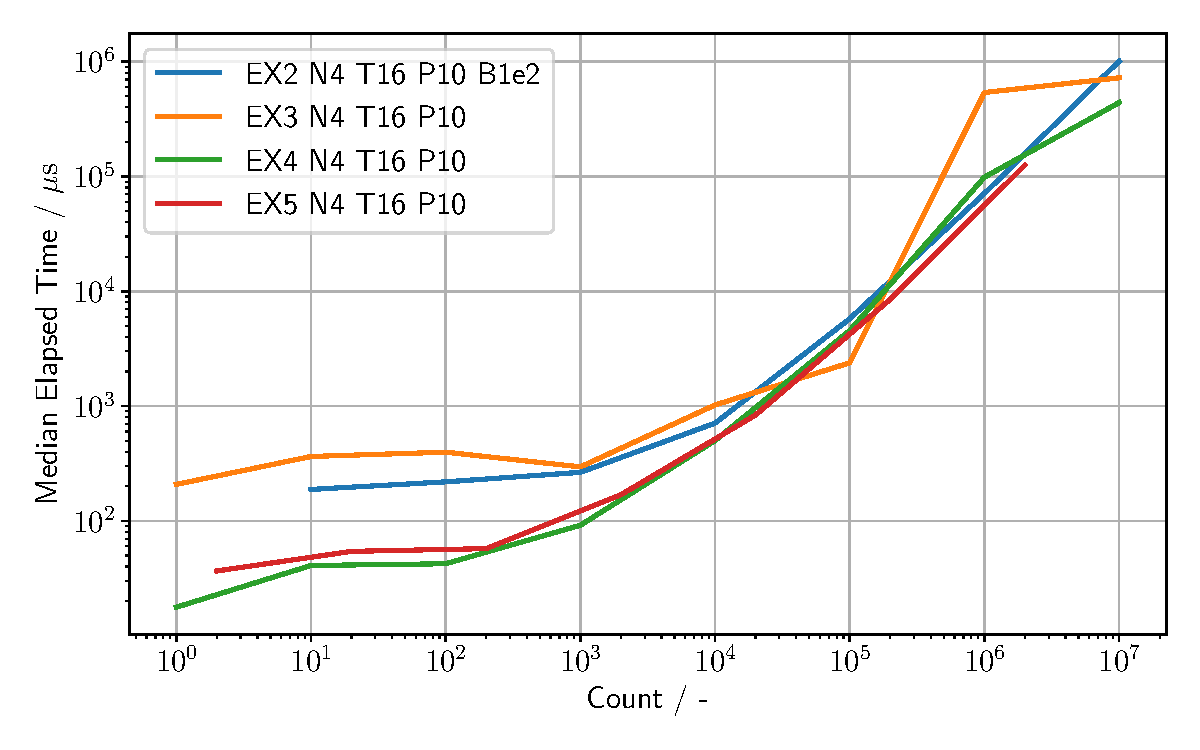
\includegraphics[width=1.0\linewidth]{figures/Ex5_3.pdf}
        \caption{Caption for Ex5 plot 3}
        \label{Ex5_3_p}
    \end{center}
\end{figure}

\begin{figure}[h]
\centering
    \begin{minipage}{.5\textwidth}
        \centering
        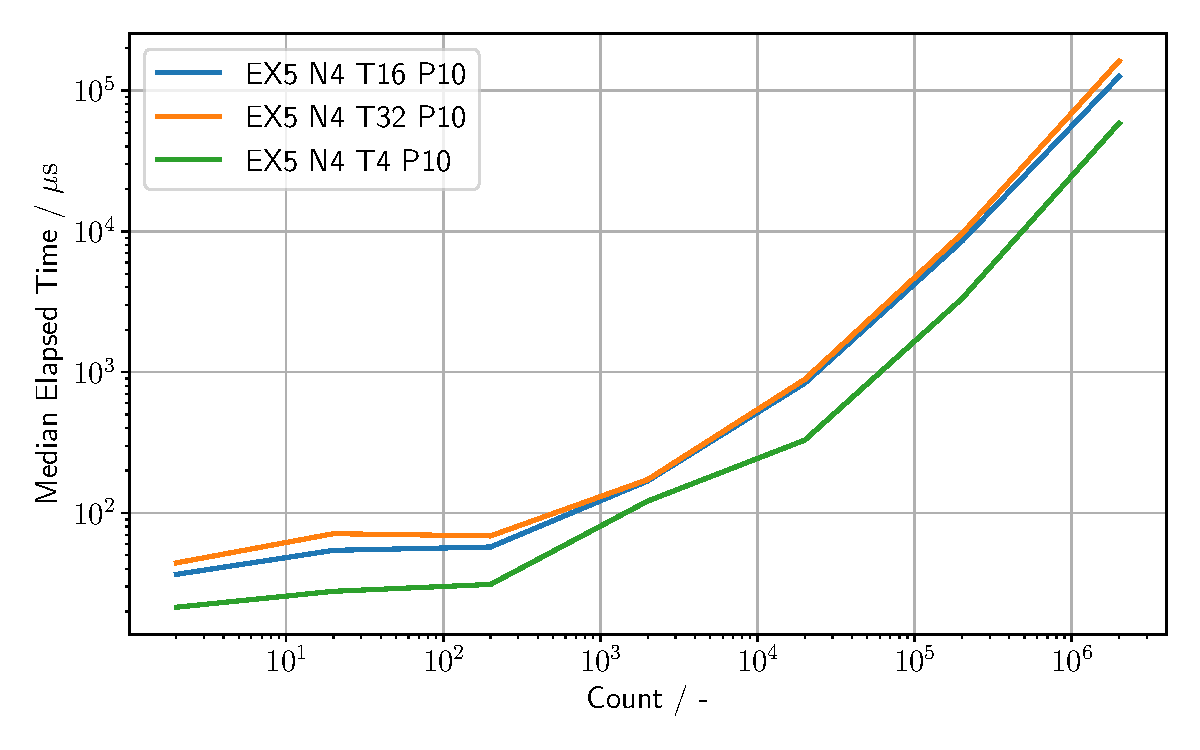
\includegraphics[width=1.0\linewidth]{figures/Ex5_1.pdf}
        \captionof{figure}{Caption for Ex5 plot 1}
        \label{Ex5_1_p}
    \end{minipage}%
    \begin{minipage}{.5\textwidth}
        \centering
        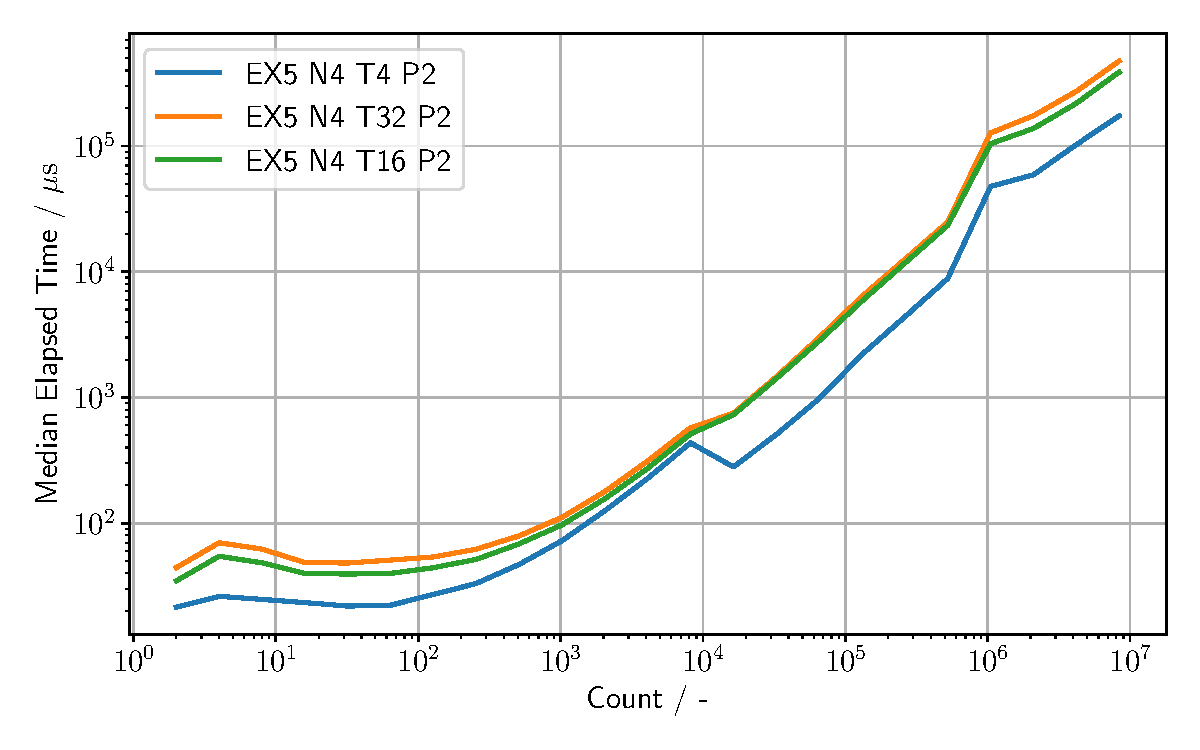
\includegraphics[width=1.0\linewidth]{figures/Ex5_2.pdf}
        \captionof{figure}{Caption for Ex5 plot 2}
        \label{Ex5_2_p}
    \end{minipage}
\end{figure}


